\documentclass[11pt,a4paper]{article}

\usepackage[margin=1.5cm]{geometry}
\usepackage[T1]{fontenc}
\usepackage{lmodern}
\usepackage{tikz}
\usetikzlibrary{automata, arrows.meta}
\pagestyle{empty}
\emergencystretch=3em

\newcommand{\co}[1]{\texttt{#1}}

% labels are anchored away from their edge, never centred on it
\tikzset{
  st/.style   = {draw, circle, minimum size=1.25cm, inner sep=1pt, font=\small},
  lb/.style   = {font=\tiny, align=left,   anchor=west,   inner sep=2pt},
  rb/.style   = {font=\tiny, align=right,  anchor=east,   inner sep=2pt},
  cb/.style   = {font=\tiny, align=center, inner sep=2pt},
  wire/.style = {->, rounded corners=5pt},
}

\begin{document}

\begin{center}
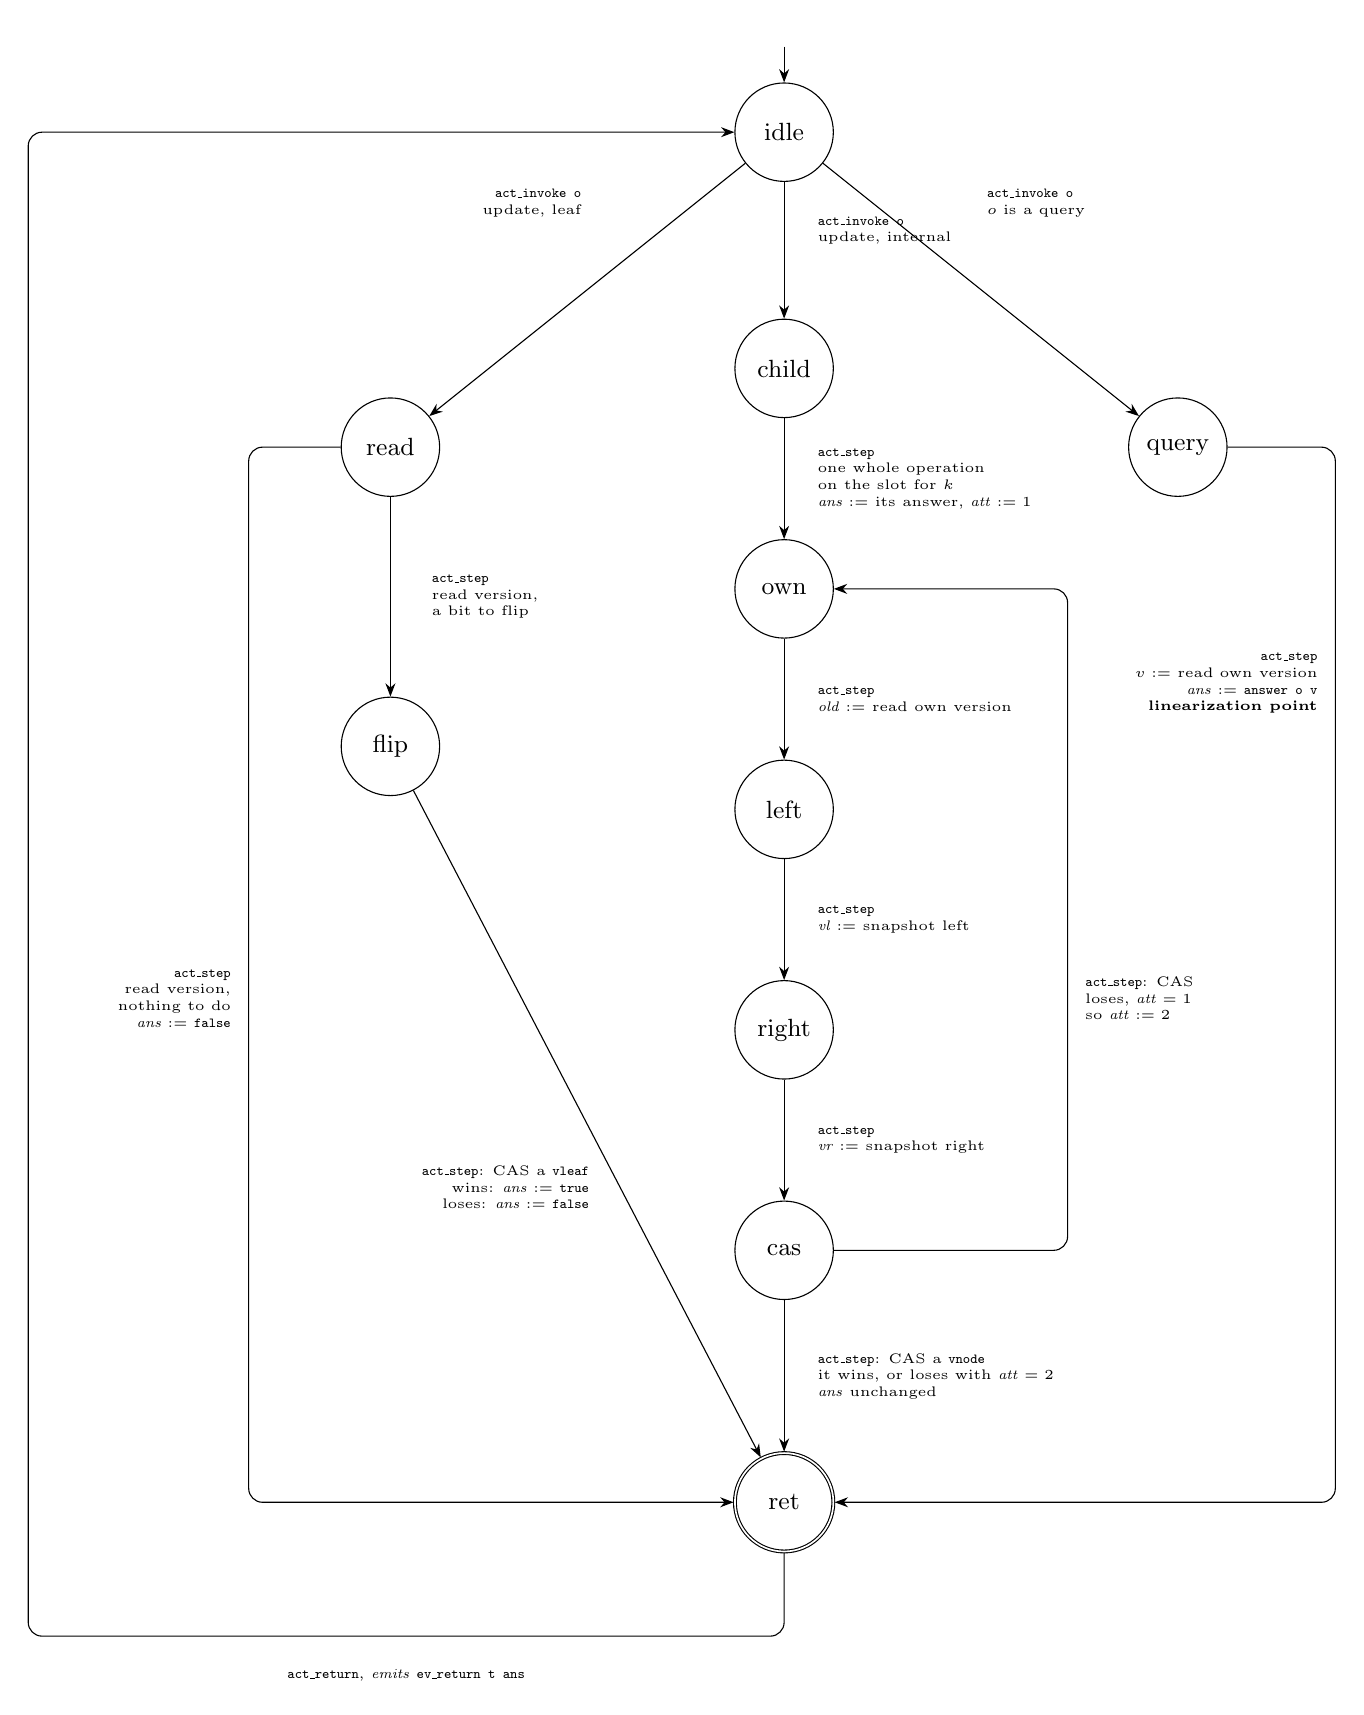
\begin{tikzpicture}[>=Stealth]

  % ===== states =========================================================
  \node[st, initial, initial where=above, initial text={}]
                       (idle)  at ( 0.0,   0.0) {idle};
  \node[st]            (read)  at (-5.0,  -4.0) {read};
  \node[st]            (flip)  at (-5.0,  -7.8) {flip};
  \node[st]            (query) at ( 5.0,  -4.0) {query};
  \node[st]            (child) at ( 0.0,  -3.0) {child};
  \node[st]            (own)   at ( 0.0,  -5.8) {own};
  \node[st]            (left)  at ( 0.0,  -8.6) {left};
  \node[st]            (right) at ( 0.0, -11.4) {right};
  \node[st]            (cas)   at ( 0.0, -14.2) {cas};
  \node[st, accepting] (ret)   at ( 0.0, -17.4) {ret};

  % ===== leaving idle ===================================================
  \draw[->] (idle) -- (read);
  \node[rb] at (-2.5,-0.9) {\co{act\_invoke o}\\ update, leaf};

  \draw[->] (idle) -- (query);
  \node[lb] at ( 2.5,-0.9) {\co{act\_invoke o}\\ $o$ is a query};

  \draw[->] (idle) -- (child);
  \node[lb] at (0.35,-1.25) {\co{act\_invoke o}\\ update, internal};

  % ===== the leaf path ==================================================
  \draw[->] (read) -- (flip);
  \node[lb] at (-4.55,-5.9) {\co{act\_step}\\ read version,\\ a bit to flip};

  \draw[wire] (read.west) -- (-6.8,-4.0) -- (-6.8,-17.4) -- (ret.west);
  \node[rb] at (-6.95,-11.0) {\co{act\_step}\\ read version,\\ nothing to do\\
                              $\mathit{ans} :=$ \co{false}};

  \draw[->] (flip) -- (ret);
  \node[rb] at (-2.4,-13.4) {\co{act\_step}: CAS a \co{vleaf}\\
                             wins: $\mathit{ans} :=$ \co{true}\\
                             loses: $\mathit{ans} :=$ \co{false}};

  % ===== the internal path ==============================================
  \draw[->] (child) -- (own);
  \node[lb] at (0.35,-4.4) {\co{act\_step}\\ one whole operation\\
                            on the slot for $k$\\
                            $\mathit{ans} :=$ its answer,
                            $\mathit{att} := 1$};

  \draw[->] (own) -- (left);
  \node[lb] at (0.35,-7.2) {\co{act\_step}\\
                            $\mathit{old} :=$ read own version};

  \draw[->] (left) -- (right);
  \node[lb] at (0.35,-10.0) {\co{act\_step}\\
                             $\mathit{vl} :=$ snapshot left};

  \draw[->] (right) -- (cas);
  \node[lb] at (0.35,-12.8) {\co{act\_step}\\
                             $\mathit{vr} :=$ snapshot right};

  \draw[->] (cas) -- (ret);
  \node[lb] at (0.35,-15.8) {\co{act\_step}: CAS a \co{vnode}\\
                             it wins, or loses with $\mathit{att} = 2$\\
                             $\mathit{ans}$ unchanged};

  \draw[wire] (cas.east) -- (3.6,-14.2) -- (3.6,-5.8) -- (own.east);
  \node[lb] at (3.75,-11.0) {\co{act\_step}: CAS\\
                             loses, $\mathit{att} = 1$\\
                             so $\mathit{att} := 2$};

  % ===== the query path =================================================
  \draw[wire] (query.east) -- (7.0,-4.0) -- (7.0,-17.4) -- (ret.east);
  \node[rb] at (6.85,-7.0) {\co{act\_step}\\ $v :=$ read own version\\
                            $\mathit{ans} :=$ \co{answer o v}\\
                            \textbf{linearization point}};

  % ===== the way home ===================================================
  \draw[wire] (ret.south) -- (0,-19.1) -- (-9.6,-19.1) -- (-9.6,0) -- (idle.west);
  \node[cb] at (-4.8,-19.6) {\co{act\_return}, \emph{emits} \co{ev\_return t ans}};

\end{tikzpicture}
\end{center}

\vspace{0.3em}

\begin{center}
\footnotesize
\begin{minipage}{0.94\textwidth}
\textbf{Key.}\;
Each circle is a value of \co{CPC}, and the italic names are the local
variables it carries: $o$ the operation, $\mathit{ans}$ the answer owed,
$\mathit{att}$ which of the two refresh attempts this is, and $\mathit{old}$,
$\mathit{vl}$, $\mathit{vr}$ the three versions a refresh reads.
Every arrow is one atomic step, one read or one CAS; a local test costs no
memory access and is decided inside the step that reaches it.
All three arrows out of \co{idle} emit \co{ev\_invoke t o} and are taken only
when \co{op\_ok i j o} holds.
Every CAS compares tags rather than shape, and the two that win consume a tag
from \co{cfresh}.
The four arrows \co{own}, \co{left}, \co{right}, \co{cas} are one
\co{refresh}, and going round them twice is the double refresh.
Any action not drawn is a stutter, leaving the configuration alone and
emitting nothing: a disallowed \co{act\_invoke}, an \co{act\_return} anywhere
but \co{ret}, and \co{act\_step} at \co{idle} or at \co{ret}.
Which of the three paths a thread takes is settled by the arrow it leaves
\co{idle} on and cannot change afterwards, so no later state retests whether
the component is a leaf; that is the lemma \co{pc\_shape\_run}.
\end{minipage}
\end{center}

\end{document}
